\documentclass[12pt, oneside]{article} 
\usepackage{booktabs}
\usepackage{geometry}              	
\usepackage{adjustbox}
\usepackage{pdfpages}  		
\usepackage{graphicx}
\usepackage{caption}						
\usepackage{amssymb}
\usepackage{amsmath}
\usepackage{pdfpages} 
\usepackage{longtable}
\usepackage{subfig}
\usepackage{url}
\usepackage{comment}

%\usepackage{subcaption}
\usepackage{graphicx}  % remove 'demo' option for your real document

\usepackage{fancyvrb}
\usepackage{hyperref}
\hypersetup{colorlinks,linkcolor={blue},citecolor={blue},urlcolor={red}}  
\usepackage{titlesec}
\usepackage{fancyhdr}
\usepackage{blindtext}
\usepackage{graphicx}
\usepackage{longtable}
\usepackage{booktabs}
\usepackage{multirow}
%\usepackage[dvipsnames]{xcolor}
\usepackage{pdflscape}
\usepackage{subfig}
\setcounter{tocdepth}{6}
\setcounter{secnumdepth}{6}
\titleformat{\paragraph}
{\normalfont\normalsize\bfseries}{\theparagraph}{1em}{}

 \setlength{\headheight}{14.5pt}
\lhead{}
 
\usepackage[english]{babel}
\usepackage[utf8]{inputenc}

\geometry{left=2.0cm,right=2.0cm,top=2.0cm,bottom=2.0cm}
%using the euro symbol
\usepackage[utf8]{inputenc}
\usepackage{marvosym}
\DeclareUnicodeCharacter{20AC}{\EUR{}}
%\usepackage[dvipsnames]{xcolor}
\usepackage{array,tabularx,calc}
%to allow use of < and >
\usepackage[T1]{fontenc}
%references
\usepackage{csquotes}
%\usepackage[style=nature]{biblatex}
%\addbibresource{references.bib}
\newlength{\conditionwd}
\newenvironment{conditions}[1][where:]
  {%
   #1\tabularx{\textwidth-\widthof{#1}}[t]{
     >{$}l<{$} @{${}={}$} X@{}
   }%
  }
  {\endtabularx\\[\belowdisplayskip]}

\usepackage{array,tabularx}

\newcommand{\HRule}[1]{\rule{\linewidth}{#1}} 	% Horizontal rule

\makeatletter							% Title
\def\printtitle{%						
    {\centering \@title\par}}
\makeatother
									

\makeatletter							% Author
\def\printauthor{%					
    {\centering \large \@author}}				
\makeatother	

\usepackage{mathtools} 

\usepackage[font=small,labelfont=bf]{caption}

\begin{document}

%\renewcommand{\labelenumii}{\Arabic{enumii}}





\begin{titlepage}
    \centering 
	\scshape
	\vspace*{2\baselineskip}
	\rule{\textwidth}{1.6pt}\vspace*{-\baselineskip}\vspace*{2pt} 
	\rule{\textwidth}{0.4pt} 
	\vspace{0.75\baselineskip} 
	{\Huge EOSC595 \\ Directed Study in Polar Climate} \\
	\vspace{0.1in}
		{\Large Literature Review} \\
		\vspace{0.1in}
		{\Large Ruth Moore} \\
	\vspace{0.75\baselineskip} 
	\rule{\textwidth}{0.4pt}\vspace*{-\baselineskip}\vspace*{2pt} 
		\rule{\textwidth}{1.6pt}
	\vspace*{2\baselineskip} 

\Huge{A review on the usage of ERA5 reanalysis in the Arctic region}
\vspace{0.1in}	

\begin{figure}[hbtp]
\centering

\includegraphics[width=0.5\textwidth]{../ubc-logo-png-transparent.png}
\end{figure}
{\Large Spring 2023- } \\
	{\large University of British Columbia} 
\end{titlepage}
\pagestyle{fancy}


{
  \hypersetup{linkcolor=black}
  \tableofcontents
}


\thispagestyle{empty}
\clearpage
\setcounter{page}{1}


\pagebreak



\section{Introduction}

{\color{blue}look at different papers which have reviewed ERA for use in other regions and base my paper off of it}


Historical measurements which are available are not evenly distributed around the globe, particularly for areas in harsh environments with small populations, such as the Arctic region. Temporal and spatial biases exist which limit complete weather measurements being taken of both the past and the present. There therefore is need for datasets which help to fill in the gaps where observations are missing.

Reanalysis data sets combine weather measurements from the past with up-to-date climate and weather models to form a complete picture of weather patterns. These data sets provide comprehensive weather and climate conditions at regular intervals overtime and are used in atmospheric dynamics, climate stability and for evaluating climate models. In many study in the Arctic region, reanalysis output are used in replacement of both historical and current measurements since the historical record is sparce.

For instance, ERA5, which forms the main body of this review, is often used as a data product when comparing CMIP (Coupled Model Intercomparison Project) model ouputs and other model outputs to 'observations'. In these cases ERA5 is used instead of observational measurements since it is a complete dataset without missing time periods or places. Examples of this include \cite{ford2022arctic} where CMIP and ERA5 are compared to evaluate hydrological changes due to sea ice loss and in \cite{rantanen2022arctic} where ERA5 data shows that the Arctic is seen to have warmed 4 times more than the global average since 1979. 

There are limitations associated with using reanalysis data.Studies using ERA5 have shown overestimations in both precipitation amount and frequency in the Arctic region.
 Therefore reanalyses output should not blindly be used as a data product without thorough evaluation of its limitations and biases within the Arctic. 

Understanding of these limitations, particularly with precipitation is crucial for work in the Arctic and for global climate evaluation as a whole. To quote Boisvert in \cite{boisvert2018intercomparison}; "[precipitation] is one of the most poorly constrained variables in atmospheric reanalyses". A large section of this review paper will focus on precipitation, since precipitation is one of the most rapidly changing variables in the Arctic as we see a transition from snow to rain, and it is one of the most limited and difficult to use reanalysis products, as will be explained in section \ref{precipitation}. This review will also look at why we use reanalysis, will discuss the major atmospheric reanalysis products available in the Arctic, introducing ERA5 as the most reliable one. Then a discussion on major variables related to the atmospheric hydrological cycle is given, where precipitation and trace precipitation are discussed in depth. Finaly a review on regional differences is given with a discussion on knowledge gaps. 


\section{Why we use reanalysis}
Reanalysis datasets ensure that we have a more thorough and robust dataset of meteorological information for the globe. They are increasingly being used in studies which look to understand climate change in certain regions, and are also used to validate other model outputs, such as CMIP5 and CMIP6. Reanalysis datasets are reliable once their limitations are understood, and provide a wide range of variables which otherwise might not be available for analysis. 

When producing reanalysis output, weather observations from the past are often assimilated. Assimilated observations are observational records which are inputted directly into reanalysis models. Interpolation and physically modelling is then done to fill in gaps in the observational record, here the state of the system is estimated using the weather models and is merged with observations to change the trajectory of the model \cite{fletcher2022data}. An example of an assimilated variable is temperature. 

If variables are not assimilated, such as precipitation, they are calculated using the weather models, with conditions provided by assimilated variables. Reanalysis is therefore similar to interpolation, however as opposed to mathematical models linking missing variable, the physics of climate and weather systems are used to fill in missing observations, and to output variables which are not available in observational records. 

Observations which are assimilated into reanalysis output include meteorological station observations, satellite measurements (such as cloud cover), radiosonde, sea level data and aircraft observations \cite{gelaro2017modern}. The satellite era is defined as the period between 1979 to present day, during which satellite data is assimilated. Using satellites results is less of a reliance on limited surface observations \cite{knutson2006assessment}, and therefore a more accurate reanalysis output.


Reanalysis products come with distinct limitations, particularly in the Arctic where assimilation is low due to limitations in observational records. Some of these limitations include a warm bias over sea ice when compared to buoy measurements \cite{wang2019comparison} and the presence of trace precipitation \cite{boisvert2018intercomparison}, this is discussed in detail in section \ref{traceprecip}.


\section{Reanalysis products available in the Arctic}

When comparing different products use a figure which looks like this 

\begin{figure}[ht]
    \centering
    \vspace{-4mm}
    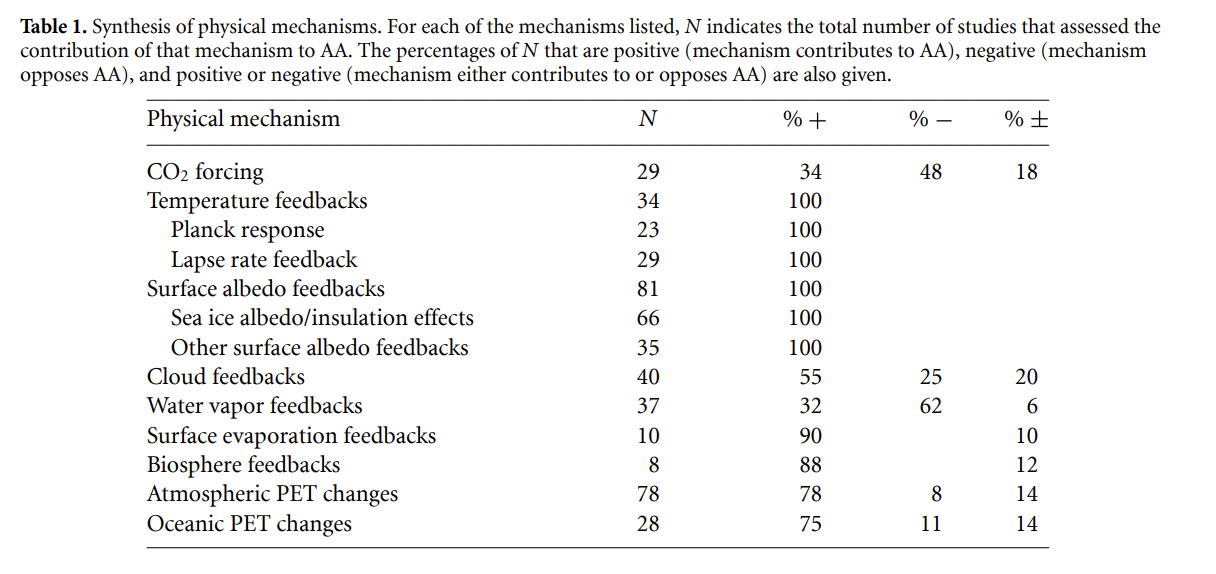
\includegraphics[width=80mm]{previdi_comparasion_mechanisms.png}
    \vspace{-4mm}
    \caption{from \cite{previdi2021arctic} }
    \label{f:previdi2021arctic}
\end{figure}




\section{An introduction to ERA5}
ERA5 is the fifth generation ECMWF (European Centre for Medium-Range Weather Forecasts) atmospheric reanalysis for the globe. The product spans from 1940 to present day and is available to download at \url{https://cds.climate.copernicus.eu/}. ERA5 provides hourly measurements for a large number of atmospheric, land and oceanic variables \cite{hersbach2020era5}. 
ERA5 grid cells are 0.25° x 0.25°, which roughly corresponds to 31km x 31km, with atmospheric resolution to 80km over 137 levels. 2D and 3D data are available with daily and monthly estimates available in addition to hourly estimates. 

ERA-5 was chosen specifically for this review as it is the most reliable global reanalysis for the Arctic right now. It has the highest correlation coefficients compared with experimental weather data, smallest biases and root-mean-square errors when compared with other reanalysis datasets \cite{graham2019improved, hillebrand2021comparison}. 

For most studies within the Arctic, only the satellite era is used for analysis, giving 44 years of output (1979-2023).




\section{An evaluation of ERA-5}
WHY IS ERA5 good?

How have other studies compared ERA5 and what have they said?

There are a number of different reanalysis datasets available for study in the Arctic. 



\section{Variables and limitations}\label{Hydrological variables and limitations }
For specific variables ERA5 is seen to perform well (such as rain on snow events in \cite{dou2021trends}). A more thorough analysis of which variables ERA5 characterizes well will be completed for this study.


\subsection{Precipitation}\label{precipitation}
%why is precipitation so hard?
As explained in \cite{boisvert2018intercomparison} Arctic wide precipitation is difficult to measure and therefore accurately reproduce. Arctic precipitation is one of the variables with the most uncertainty in forecasting and global climate projections. 

\subsubsection{ERA5 trace precipitation}\label{traceprecip}
Most observational stations in the Arctic record precipitation to the nearest 0.1mm/day, with any precipitation less than 0.1mm/day being considered trace. This is because amounts less than 0.1mm/day are incredibly difficult to measure using rain gauges \cite[p.~3-50]{meteorological2015manobs}. A large number of trace precipitation values exist in ERA5 precipitation output, which do not exist in observational records \cite{shen2022performance}. This is because reanalysis products are generally oversensitive to microphysical and atmospheric dynamics on a global scale \cite{boisvert2018intercomparison}. 


particularly focusing on precipitation as it is relevant to my work
\section{Regional differences}
Some studies have looked at specific regions, comparing how well ERA5 performs with extreme events \cite{loeb2022extreme} in Western Canada and Greenland. This review will compare specific regions where ERA5 has been evaluated.


\section{Knowledge gaps}


\section{Conclusion}

Reanalysis models also often have biases due to changing observation methods. This aside, they are useful and critical to researching climate in the recent past. 




 \bibliography{../mybib}{}
\bibliographystyle{apalike}

\end{document}


